\documentclass{article}
\usepackage{graphicx}
\usepackage{float}
\parskip=12pt

\begin{document}

\title{Laboratory 4: DC and AC Circuits}
\date{November 19, 2014}
\author{Calvin Chan\\304144970\\Physics 4BL Lab 8\\Partners: Caleb Choi, Stanley
Chan}

\maketitle

\section{Introduction}

This lab aims to demonstrate, through experimental calculations, the speed of
sound and light by analyzing the different properties of waves (standing and
otherwise). The speed of sound will be measured through the analysis of angular
frequency and its relationship with the wave number and wave lengths. Similarly,
the speed of light will be measured through the analysis of various maximuma and
minima in standing waves to calculate wavelength, and furthermore, the velocity
of light.

\section{Experimental Results}

\subsection{Dispersion Relation for Sound Waves}

The first part of the lab aims to demonstrate the relationship between angular
frequency of a sound wave and its wave vector, or wave number. This relationship
should yield the velocity of the wave itself because of the following equation:

\begin{equation}
    \label{phase_velocity}
    v_{p}=\frac{\omega}{k}
\end{equation}

\begin{enumerate}
    \item Place a microphone and a speaker on a linear track and capture data
    \item Experiment with different distance deltas between the microphone and
    the speaker
    \item Note the distances where the phase transitions from 0 to $2\pi$
\end{enumerate}

Having obtained 5 different data sets with angular frequency and the wavevector
(calculated using the wavelength), we can proceed to plot each data set to form
a representation of the wave velocity.

\begin{figure}[H]
    \centering
    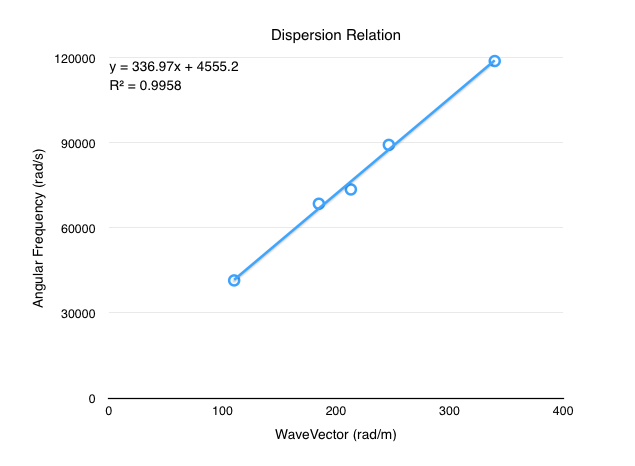
\includegraphics[width=\textwidth]{charts/dispersion_relation}
    \caption{The dispersion relation for traveling sound waves}
    \label{dispersion_relation}
\end{figure}

\subsection{Wavelengths of Standing Sound Waves}

The second section of the lab aims to demonstrate the various properties that
standing waves exhibit and use them to measure the wavelength of standing waves.
By measuring continuous maxima and minima, we can determine the length of half a
wavelength, and essentially the wavelength of a standing wave.

\begin{enumerate}
    \item Use a reflector to generate different standing waves with different
    wave lengths.
    \item Using the potentiometer, measure the voltage generated by each
    standing wave
    \item Make note of the maxima and minima voltage exhibited by each standing
    wave.
\end{enumerate}

We had the microphone output a frequency of $6.6kHz$. We calibrate the
potentiometer to convert voltage into distance by measuring the voltages at
different distance deltas where the distance delta is a known constant.

\begin{figure}[H]
    \centering
    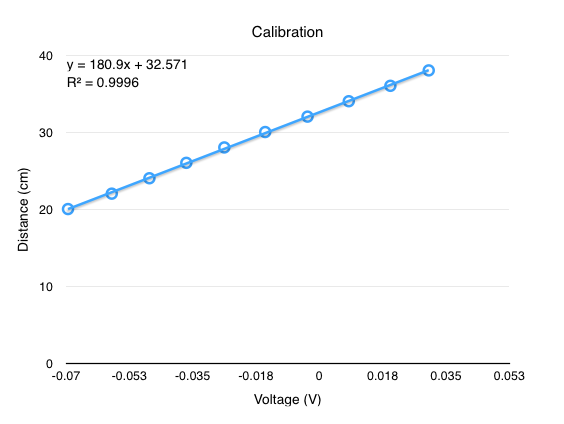
\includegraphics[width=\textwidth]{charts/calibration}
    \caption{A calibration plot to map the coefficient relation between distance
    and voltage}
    \label{calibration}
\end{figure}

Using the slope of the calibration plot ($m=180.9$), we can map the recorded
voltage for CH.0 to distance. Plotting the distance against the sound voltage
from CH.1, we get the following graph:

\begin{figure}[H]
    \centering
    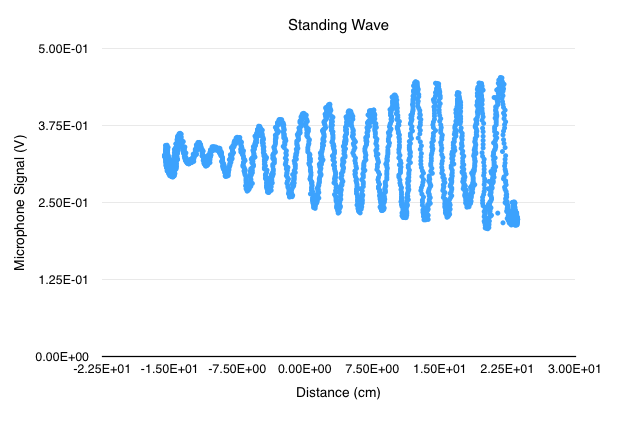
\includegraphics[width=\textwidth]{charts/standingwave_sound}
    \caption{A plot of the sound standing wave}
    \label{standingwave_sound}
\end{figure}

We can isolate the maxima and minima to calculate the wavelength of the standing
wave. From fig. \ref{sound_wavelength}, we can calculate the average value of
the wavelength to be $\lambda = 2.44cm$. With a standard deviation of $0.197$
and a total of $8$ measurements, we can calculate the standard deviation of the
mean to be $0.0698$.

\begin{figure}[H]
    \centering
    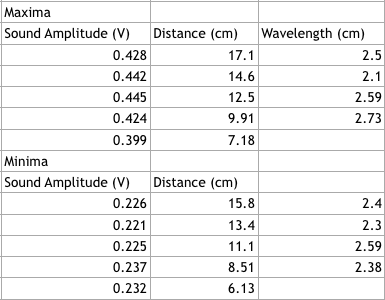
\includegraphics[width=0.5\textwidth]{charts/sound_wavelength}
    \caption{A chart of 5 different maxima and minima sound voltage values}
    \label{sound_wavelength}
\end{figure}

\subsection{Wavelengths of Standing EM Waves}

Similar to the previous part of the lab, we want to determine the wavelength of
a standing wave, except this time, it is an EM wave instead of a sound wave. We
use a cordless phone to generate the EM waves and place a Yaqi antenna between
the phone and a moveable reflector. By moving the reflector, we can generate a
standing wave with several maxima and minima. The result is shown in figure
\ref{standingwave_em}

\begin{figure}[H]
    \centering
    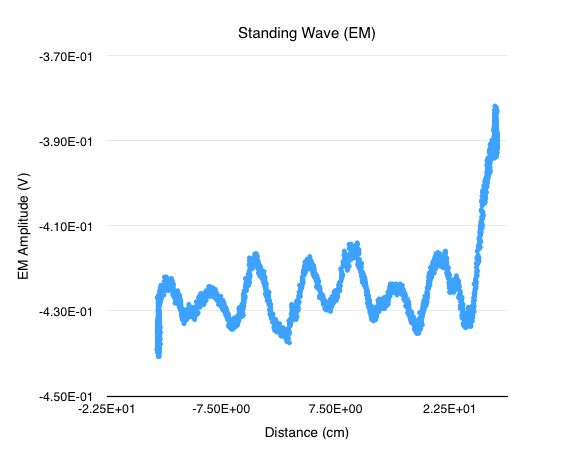
\includegraphics[width=\textwidth]{charts/standingwave_em}
    \caption{A plot of the em standing wave}
    \label{standingwave_em}
\end{figure}

Once again, we can isolate the maxima and minima to calculate the wavelength of
the standing wave. The maxima and minima are shown as a chart in figure
\ref{em_wavelength}.

\begin{figure}[H]
    \centering
    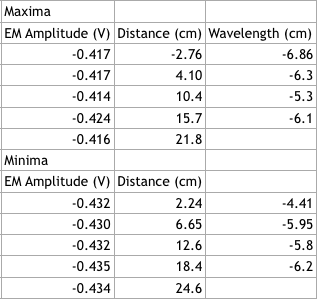
\includegraphics[width=0.5\textwidth]{charts/em_wavelength}
    \caption{A chart of 5 different maxima and minima EM voltage values}
    \label{em_wavelength}
\end{figure}

\section{Analysis}

\subsection{Dispersion Relation for Sound Waves}

Through the linear regression performed on the model represented by figure
\ref{dispersion_relation}, we can see that the experimental value for the speed
of sound in air is $336.97\frac{m}{s}$ with an outputted standard error of
$37.161\frac{m}{s}$.

Comparing our experimental value to the actual value of the speed of sound in
air at room temperature ($343.2\frac{m}{s}$), we see that there is an error of
$6.23\frac{m}{s}$, which falls well within the error yielded by our linear
regression.

\subsection{Wavelengths of Standing Sound Waves}

From fig. \ref{sound_wavelength}, we can calculate the average value of
the wavelength to be $\lambda = 2.44cm$. With a standard deviation of $0.197$
and a total of $8$ measurements, we can calculate the standard deviation of the
mean to be $0.0698$.

From our calculations, the experimental value of the average wavelength is
$\lambda = 2.44\pm 0.0698 cm$. Given $f=6.6kHz$, which was the frequency that we
used for this part of the lab, and using the experimental value of $\lambda$, we
can calculate the speed of sound, as well as its uncertainty.

\begin{equation}
    \label{vflambda}
    v = f\lambda
\end{equation}
\begin{equation}
    \label{vflambda_sound1}
    v = (6.6kHz)(2\cdot0.0244)
\end{equation}
\begin{equation}
    \label{vflambda_sound2}
    v = 351.35 \frac{m}{s}
\end{equation}

Using the error propogation formula, we can calculate the uncertainty of our
experimental $v$ of sound, which turns out to be $14.86\frac{m}{s}$.

Comparing our experimental value to the actual value of the speed of sound in
air at room temperature ($343.2\frac{m}{s}$), we see that there is an error of
$8.15\frac{m}{s}$, which falls within the error yielded by our error propogation
calculations.

\subsection{Wavelengths of Standing EM Waves}

From fig. \ref{em_wavelength}, we can calculate the average value of
the wavelength to be $\lambda = 5.87cm$. With a standard deviation of $0.736$
and a total of $8$ measurements, we can calculate the standard deviation of the
mean to be $0.261$.

From our calculations, the experimental value of the average wavelength is
$\lambda = 5.87\pm 0.261 cm$. Given $f=2.4GHz$, which was the frequency of the
phone that we used for this part of the lab, and using the experimental value of
$\lambda$, we can calculate the speed of light, as well as its uncertainty.

\begin{equation}
    v = f\lambda
\end{equation}
\begin{equation}
    \label{vflambda_em1}
    v = (2.4GHz)(2\cdot0.0587)
\end{equation}
\begin{equation}
    \label{vflambda_em2}
    v = 2.82 \cdot 10^{8} \frac{m}{s}
\end{equation}

Using the error propogation formula, we can calculate the uncertainty of our
experimental $v$ of light, which turns out to be $7.30 \cdot 10^{7}
\frac{m}{s}$.

Comparing our experimental value to the actual value of the speed of light in
($3.00\cdot10^{8}\frac{m}{s}$), we see that there is an error of
$1.8\cdot10^{7}\frac{m}{s}$, which falls within the error yielded by our error
propogation calculations.

\section{Conclusion}
This experiment successfully demonstrated properties of sound waves and light
waves. We successfully calculated the speed of sound within the uncertainties
and errors that propogated through the experiment using the relationship between
angular frequency and wave vector. Furthermore, our calculations using the
standing waves for both sound and light were close to the actual values of the
speeds of sound and light, with errors falling within the threshold yielded
by error propogation.
\end{document}
